\chapter{Convolutional Nets}
% Authors: Fekade Brook, Nicholas Greenquist, Aaron Wong
% Lecture date: 2/11/2019

\section{Parameter Space Transform}
% Authors: Fekade Brook, Nicholas Greenquist, Aaron Wong
% Lecture date: 2/11/2019

Weights of a neural net do not necessarily have to be parameters. 
They can be outputs of other functions.

\begin{figure}
    \centering
    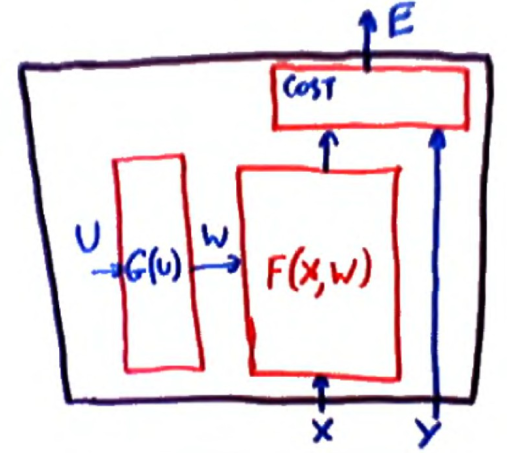
\includegraphics[width=150pt]{lectures/03-a/images/parameterize.png}
    \caption{Re-parameterization of weight parameters U}
    \label{fig:param}
\end{figure}

For example, in \cref{fig:param} the parameters of $F$ are $W$ but $W$ are not the parameters that you learn. 
The parameters that you learn are the $U$ but these are re-parameterized by a function $G:U\rightarrow W$ before being sent to $F$. 
This is only simple example of re-parameterizing. 
We could also have a function that re-paramterizes the inputs $X$.

If you use the functional form of PyTorch this is very easy to do. 
Everything works when you backpropagate. 
To use the above figure as an example again, when you back propagate you get the gradient of the cost with respect to the $F$ module. 
Backpropagating even further gives you the Jacobian of $F$ module times the Jacobian of the $G$ module. 
The nice thing is that if you use PyTorch, all of the gradients and backpropagation is handled for you and you do not need to think about it. 

\section{Weight Sharing}
% Authors: Fekade Brook, Nicholas Greenquist, Aaron Wong
% Lecture date: 2/11/2019

\Cref{fig:sharing} is an example of a function $G$ that can be used to re-parameterize the weight parameters.

\begin{figure}
    \centering
    \includegraphics[width=150pt]{lectures/03-a/images/weight_sharing.png}
    \caption{Weight sharing of weights $w_{i}$}
    \label{fig:sharing}
\end{figure}

In this example, $G$ replicates a single parameter multiple times and passes the new parameters to $F$. 
When we backpropagate, the gradient with respect to that shared parameter is equal to the sum of the gradients with respect to each of the replicated parameters.

\section{Mixture of Experts}
% Authors: Fekade Brook, Nicholas Greenquist, Aaron Wong
% Lecture date: 2/11/2019

If we have a function that works well in restricted domains of the input space but does not work globally, we want to create something that is called a Mixture of Experts. 
This idea of combining multiple, local optimal functions allows for very interesting architectures. 
This idea is actually the inspiration behind attention mechanisms that we will see later. 

Imagine you have a problem with 3 distinct types of inputs. 
An example is recognizing faces. 
You might need a different model for children, male adults, and female adults. 
You would want 3 expert models for each of those types.

Visually, we can see that this input would benefit from 3 separate classifiers that we can combine in \cref{fig:mixture}

\begin{figure}
    \centering
    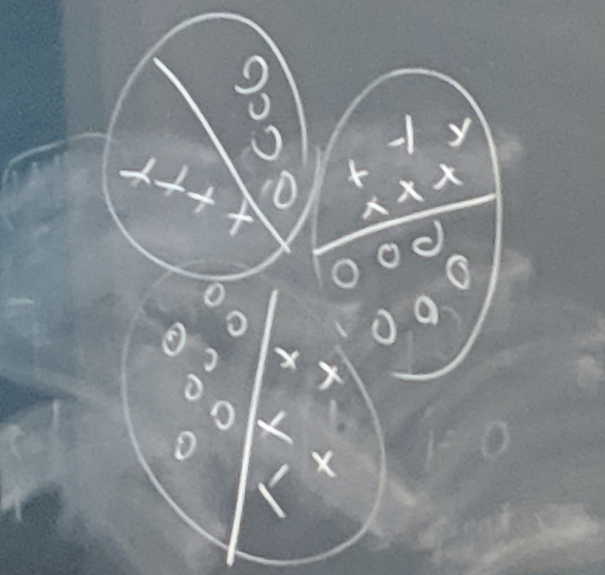
\includegraphics[width=200pt]{lectures/03-a/images/mixture.png}
    \caption{Mixture of 3 separate classifiers}
    \label{fig:mixture}
\end{figure}

The goal is to turn non-linear problems into a mixture of multiple linear classifiers. 
The mixture's sole job is to now decide where the regions are. 
Often times each of the expert systems is a neural net itself and is combined using a neural net to decide optimal region splitting. 
Softmax is often used as the final layer of a neural network for classification. 
These models can be trained with backpropagation just like what we have seen so far. 

A good example of this is speech recognition. 
Imagine I want a model to work on German, French, and English. 
I don't want to create 3 different models. 
Instead I can let the model decide which language it is dealing with and then pass the sequence into different expert systems. 
However, in reality, the input does in fact go through all of the systems, and so we use a ``Gater'' module to decide which expert to believe. 
This is all done by how our weights are tuned and how they behave with certain types of inputs. 
As usual, the modules are trained using backpropagation. 
This includes the Gater module.

\section{Time Delayed Inputs}
% Authors: Fekade Brook, Nicholas Greenquist, Aaron Wong
% Lecture date: 2/11/2019

Let's say we want to apply a neural network to a sequence of vectors. 
We want to use an input that is a "time window''. 
That is, we want to do time series predictions.

For example, you are a power company and you want to predict what the power consumption is going to be for different areas. 
The input is obviously historical power consumption and weather but you might also have time of day. 
Time-Delayed inputs are also heavily used in the financial markets. 

\begin{figure}
    \centering
    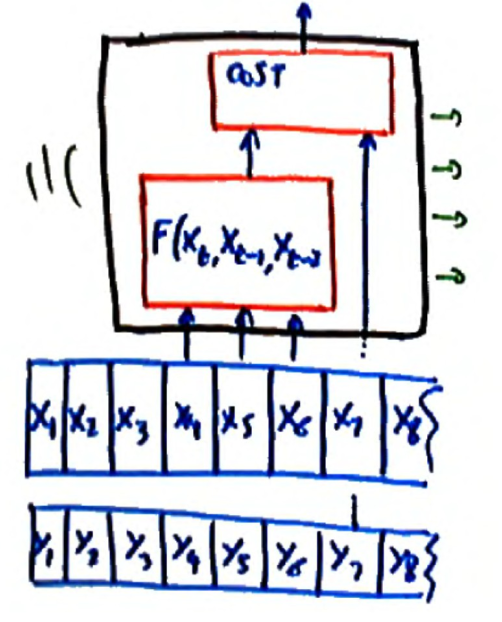
\includegraphics[width=150pt]{lectures/03-a/images/td_inputs.png}
    \caption{Neural network for time-delayed inputs}
    \label{fig:td_inputs}
\end{figure}

To do this, we feed the neural network a recent window of observed values and ask it to predict the next value. 
During training, the output at time step $t$ is usually the input at time step $t+1$ as in \cref{fig:td_inputs}. 
The motivation for this is that like in financial markets, the thing that you want to predict has already been observed. 
You just want to predict when it will happen in the future. 
The basic technique is to take our network and ``slide'' it across the inputs. 
The same weights end up getting applied to multiple inputs in the input sequence. 

An example of using time-delayed inputs is using a neural network for sound recognition on speech. 
Suppose you have a speech signal and you want to train a neural network to figure out what sound is being pronounced at the moment. 
After some pre-processing of the sound, the neural network looks at a small window of the signal. 
The network gives you a score for every possible sound that can exist. 
Slide the network over the input sequence by 10 milliseconds or so and repeat. 
Now for every 10 millisecond, you have a vector of scores for what sound is being pronounced.

\section{1D Temporal Convolutional Net}
% Authors: Fekade Brook, Nicholas Greenquist, Aaron Wong
% Lecture date: 2/11/2019

The idea we saw before of sliding the same network across different areas of the input leads to the idea of convolutions. 

Image we have the 2-layer network as shown in \cref{fig:2layer}. 
It is trying to recognize, classify or predict something from $x_{1,t}, x_{2,t}$ input sequences. 
The first layer is a single linear layer. 
Each of $C_{1}, C_{2}, C_{3}, C_{4}$ are shifted versions of the linear layer looking at different time steps of the inputs $x_{1,t}, x_{2,t}$. 
Take for instance $C_{1}$.
$C_{1}$ consists of a bunch of units each looking at a $2\times 3$ grid of the input.
After the first iteration, take those same units and shift them by one time step so that the units are now looking at a $2\times 3$ grid shifted to the right by 1.
$C_{2}$ represents this newly shifted set of units.
This is done until all the inputs are looked at.
The second layer then does something similar.
For example, in \cref{fig:2layer}, $L2$ takes three different time steps of the outputs of the units in $C_{1}, C_{2}, C_{3}, C_{4}$ and produces an output.
The important part to note here is that $C_{1}, C_{2}, C_{3}, C_{4}$ all contain the same units.
They are just the units at different time steps.

\begin{figure}
    \centering
    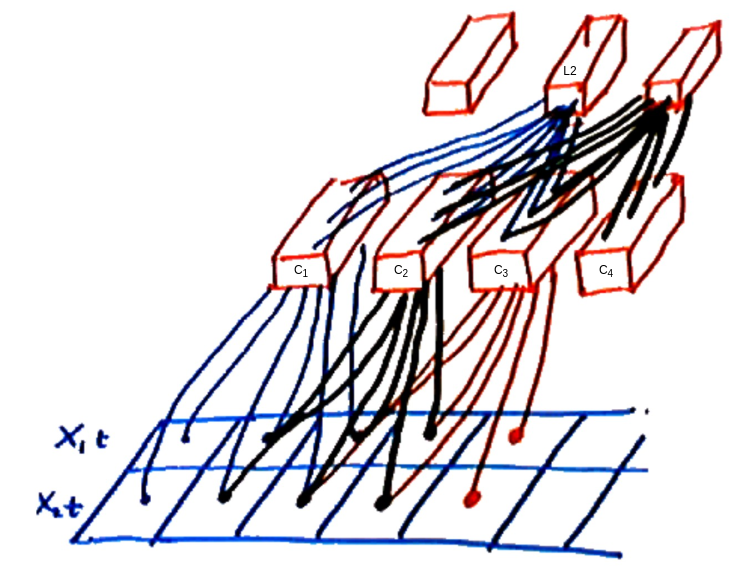
\includegraphics[width=200pt]{lectures/03-a/images/conv_net.png}
    \caption{1D (temporal) ConvNet}
    \label{fig:2layer}
\end{figure}

The idea of shared weights is that many of the weights in each layer are exactly the same but used in different time steps. 
As you train a network like this many of the parameters are used to compute values across different time steps so when you backpropagate, you need to compute the gradient of the same weight at each time step, add them up and then update that common weight with that gradient.

\subsection{2D Temporal Convolutional Net}
% Authors: Fekade Brook, Nicholas Greenquist, Aaron Wong
% Lecture date: 2/11/2019

\begin{center}
    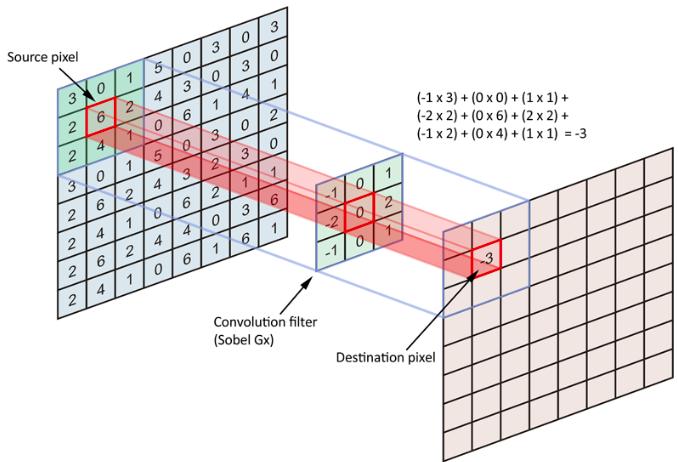
\includegraphics[width=200pt]{lectures/03-a/images/conv.png}
\end{center}

As you can see from the image above, that single filter has 9 weights. However, we slide that filter across the entire input grid. So, those 9 weights are shared to compute many different output values destination grid. When training a network with convolution like this, we need to keep track that each weight is being used multiple times and combine the gradients correctly. 
